\documentclass{article}
\usepackage[cm]{fullpage}
\usepackage{graphicx}

\author{Adeesha Ekanayake}
\title{Report: Dana Internship}

\begin{document}

\maketitle

\section{Description: }
For my DANA internship, I aimed to create a framework to create games which help people with motor difficulty improve their motor skills. This system would use the Microsoft Kinect sensor to detect and track the movements of patients, allowing them to interact with games using their body as a controller. To create the system, I used the Unity Game Engine, as well as the Zigfu library for Microsoft Kinect. 

In the fall of 2011, I undertook Independent Study with Dr. Sharon Stansfied of the Department of Computer Science at Ithaca College. This research project was aimed at exploring the capability of the Microsoft Kinect to create such a system, to help individuals with motor difficulties to improve their motor skills. During that time, I was able to create a simple game using the Microsoft XNA game development system which used the hand of a player to move a spaceship in a 2d game space. 

By creating this simple game I was able to learn a lot about the capabilities of the microsoft Kinect, and with Dr. Stansfield's support, I wanted to further explore the capabilites of the Kinect. During the Spring of 2012, I, along with a group of friends including Aaron Mansur (Clinical Health Studies 2014) attempted to create a full-featured game as an entry for the Microsoft Imagine Cup of 2012. Unfortunately, we were not able to create such a game not only because of the difficulty of using the Microsoft Kinect SDK to create our system, but also because of the lack of existing kinect-based gesture recognition frameworks on which to base our game. 

For my DANA internship, under the guidance of Dr. Stansfield, I created a simple framework on which to base a future game. The framework consisits of a set of Unity Scripts coded in C\#, as well as a therapist's interface and a very simple game to demonstrate the framework's capabilities. The therapist's interface (Figure ~\ref{Gameshot2}) is a Unity executable which is designed to allow a therapist to record an exercise, mark key poses in the exercise and save it. The game is a simple implementation of the children's game ``Simon Says,'' (Figure ~\ref{Gameshot}) where a character in-game assumes a sequence of poses which the patient must follow. As the patient follows each pose, the game detects whether or not he or she is assuming the correct pose and responds accordingly. In order to improve the patient's awareness of his or her posture, the player's avatar appears on-screen and assumes the posture of the player in real-time.

\begin{figure}[htb]
	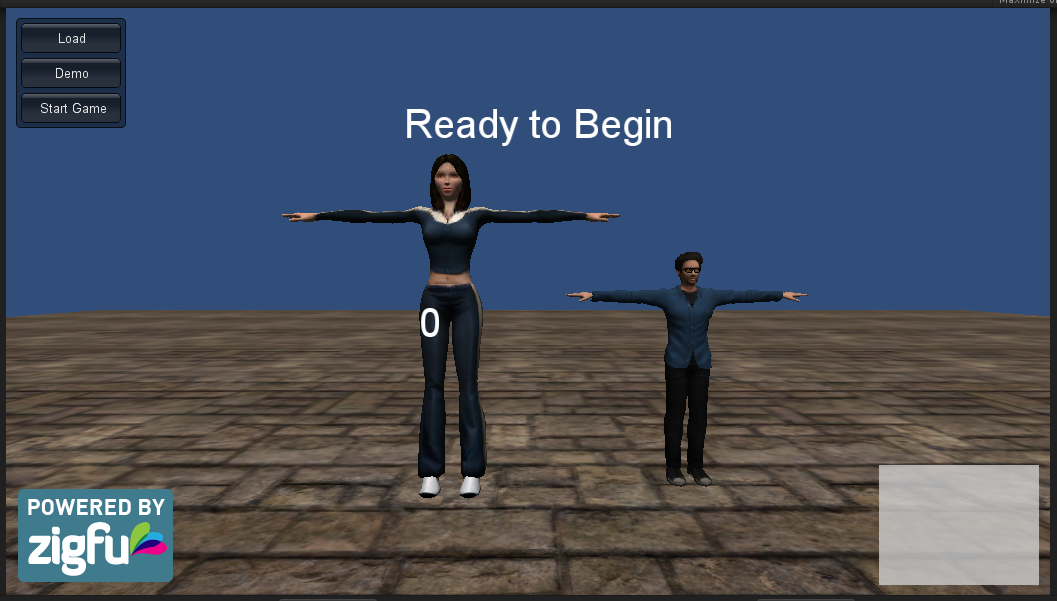
\includegraphics[width=\linewidth]{Game.png}
	\caption{Screenshot of the Game}
	\label{Gameshot}
\end{figure}

\begin{figure}[htb]
	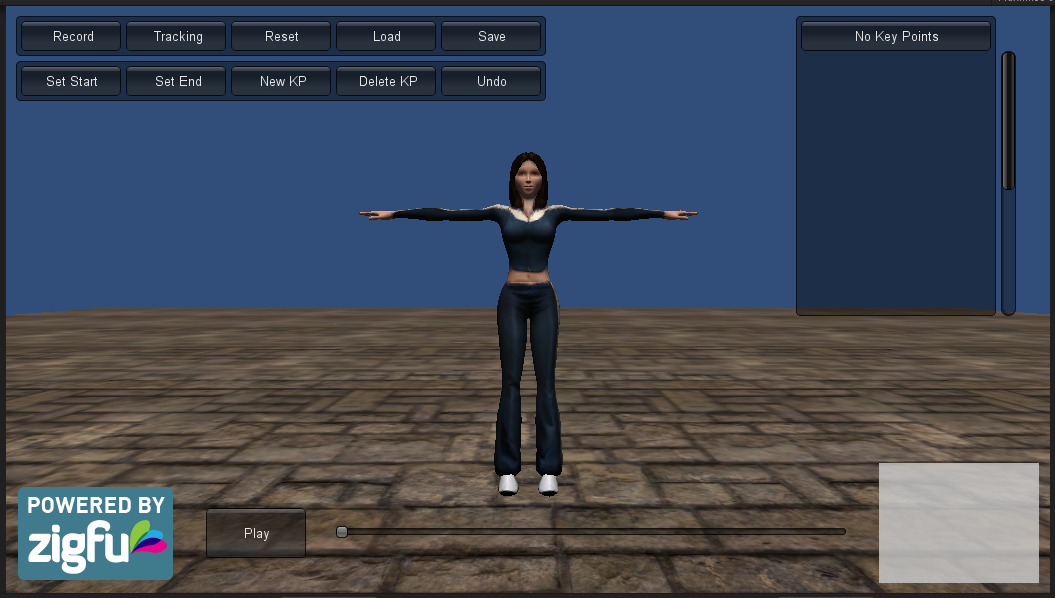
\includegraphics[width=\linewidth]{TherapistsInt.png}
	\caption{Screenshot of Therapist's interface}
	\label{Gameshot2}
\end{figure}

\paragraph{Tools and Environments}
To create this system, I made use of the following tools
\begin{itemize}
	\item \textbf{Unity3d} This is the game engine I used. Unity3d is widely used among independent game developers, and is widely recognised to be powerful and extensible.

	\item \textbf{Zigfu} This library allows developers to use the Microsoft Kinect with Unity3d. 

	\item \textbf{Microsoft Kinect} This powerful sensor package was developed by Microsoft for use with the Xbox360 game system in order to allow users to interact with games using only their body as a controller. This system has been widely used for research purposes because it includes a powerful set of sensors into an affordable package
\end{itemize}

\section{Significant Challenges}
In the course of my internships, I ran into the following significant challenges:
\begin{itemize}
	\item \textbf{Lack of GUI support in Unity} Graphical User Interfaces, or GUIs, are sets of visual controls such as buttons, lists, checkboxes, etc, which allow users to graphically interact with systems in a standardised and intuitive way. Unfortunately, Unity3d does not have a powerful built-in GUI system. 

	\item \textbf{Lack of Documentation in Zigfu} Zigfu is still in relatively early stages of development, and therefore, it is not well documented. Most of the code I made use of from the Zigfu Library was entirely undocumented, which made adadpting Zigfu code difficult.

	\item \textbf{Lack of a suitable Gesture Engine} A Gesture detection engine is used to detect and recognise user gestures to allow users to interact with a system. Unfortunately, there is no publicly available Gesture Recognition system for use with Unity3d, which would be suitable for detecting poses. 
\end{itemize} 

During the course of my internship, here is how I faced the above challenges:

\begin{itemize}
	\item \textbf{Created my own GUI framework} Using the rudimentary GUI system available in Unity3d, I was able to create a more powerful set of GUI tools for use with my game framework. 

	\item \textbf{Studied undocumented code} Since the Zigfu library was mostly undocumented, I had to peruse the source code of many of the Zigfu source files and understand what the Zigfu libraries do. In order to do so, I also made use of online resources such as user groups and forums.

	\item \textbf{Created my own gesture recognition engine} Using basic principles shared by other developers online, I was able to create my own gesture recognition system for Kinect. This system is particularly tailored to my game framework, and is based on measuring the total deviation between equivalent limb transforms. 
		
\end{itemize}

\section{Advantages and limitations of my System}

The following are some of the primary advantages and disadvantages of my system.

\paragraph{Limitations}

\begin{itemize}
	\item \textbf{Jitter} Skeletal tracking using the Microsoft Kinect is not perfectly precise; in the skeletal tracking stream from the kinect software, there is considerable noise. Both the Kinect software and my own gesture tracking software are designed to mitigate the effects of this noise but gesture tracking is still not perfect. However, the tracking software is under continuous development, and as it improves, jitter will decrease, making the system more and more precise.

	\item \textbf{Game is too simple} The game I created for demonstration purposes is far too simple for real-world use. However, in future I hope to use my game framework to create a full-featured game which helps improve individuals with motor difficulties improve their motor skills through exercise.
\end{itemize}

\paragraph{Advantages}

\begin{itemize}
	\item \textbf{Cheap and powerful Hardware} The Microsoft Kinect sensor package currently costs only \$149.99, while other similar sensor systems currently used to help individuals with motor difficulty routinely cost thousands of dollars. Therefore, this system enjoys a major cost advantage.

	\item \textbf{More precise movement} By monitoring and tracking a patient's movements, this system can potentially improve home exercise regimens for patients who need physical therapy by a large margin. 
\end{itemize}

\section{Further plans}
Now that I have completed the framework, I hope to use it to create a full-featured game for people with motor difficulties. I hope to add the following features to this game

\begin{itemize}
	\item Feedback to care provider: The game will have a system for tracking and monitoring a patient's progress with exercises over time, and automatically transmitting it to the care provider.

	\item Automatic transmission of Files: Once the therapist records an exercise, it can be transmitted automatically to the patient

	\item Full-featured game: The game will have a high production value approaching that of a commercially available video game
\end{itemize}

\end{document}
